% Use the following line _only_ if you're still using LaTeX 2.09.
%\documentstyle[icml2017,epsf,natbib]{article}
% If you rely on Latex2e packages, like most moden people use this:
\documentclass{article}

% use Times
\usepackage{times}
% For figures
\usepackage{graphicx} % more modern
%\usepackage{epsfig} % less modern
\usepackage{subfigure}
\usepackage{caption}
\usepackage{xcolor,colortbl}

% For citations
\usepackage{natbib}

% For algorithms
\usepackage{algorithm}
\usepackage{algorithmic}
\usepackage{amssymb}
\usepackage{amsmath}
% As of 2011, we use the hyperref package to produce hyperlinks in the
% resulting PDF.  If this breaks your system, please commend out the
% following usepackage line and replace \usepackage{icml2017} with
% \usepackage[nohyperref]{icml2017} above.
\usepackage{hyperref}

\usepackage{array}
\usepackage{booktabs}
% Packages hyperref and algorithmic misbehave sometimes.  We can fix
% this with the following command.
\newcommand{\theHalgorithm}{\arabic{algorithm}}

% Employ the following version of the ``usepackage'' statement for
% submitting the draft version of the paper for review.  This will set
% the note in the first column to ``Under review.  Do not distribute.''
\usepackage[accepted]{icml2017}

% Employ this version of the ``usepackage'' statement after the paper has
% been accepted, when creating the final version.  This will set the
% note in the first column to ``Proceedings of the...''
%\usepackage[accepted]{icml2017}


% The \icmltitle you define below is probably too long as a header.
% Therefore, a short form for the running title is supplied here:
\icmltitlerunning{Classifying 3-Dimensional Shapes}
\begin{document}

\twocolumn[
\icmltitle{Classifying 3-Dimensional Shapes with \\
           Convolutional Neural Networks (CS 760 2017)}

% Authors
\icmlsetsymbol{equal}{*}

\begin{icmlauthorlist}
\icmlauthor{David Porfirio}{wisc}
\icmlauthor{Andrew Schoen}{wisc}
\icmlauthor{Lorenzo Najt}{wisc}
\icmlauthor{Krittisak Chaiyakul}{wisc}
\icmlauthor{Junda Sheng}{wisc}
\end{icmlauthorlist}

\icmlaffiliation{wisc}{University of Wisconsin, Madison, Wisconsin, USA}
\icmlcorrespondingauthor{Andrew Schoen}{aschoen2@wisc.edu}
\vskip 0.3in
]

% this must go after the closing bracket ] following \twocolumn[ ...

% This command actually creates the footnote in the first column
% listing the affiliations and the copyright notice.
% The command takes one argument, which is text to display at the start of the footnote.
% The \icmlEqualContribution command is standard text for equal contribution.
% Remove it (just {}) if you do not need this facility.

%\printAffiliationsAndNotice{}  % leave blank if no need to mention equal contribution
%\printAffiliationsAndNotice{\icmlEqualContribution} % otherwise use the standard text.
%\footnotetext{hi}

\begin{abstract}
We investigate various parameters for the structure and implementation of Convolutional Neural Nets (CNNs),
offering insights into the capabilities and limitations of such algorithms in the space of 3-dimensional shape recognition.
In particular, we train and test 3-dimensional spheres and tori that have undergone a range of standard distortions.
Our results indicate that such a task is clearly possible for some collections of individual distortions,
but further work is needed to improve classification accuracy on composites of distortions, and to elucidate the
precise features learned by such systems in this domain.
\end{abstract}

\section{Introduction and Motivation}
Humans have evolved a complex classification scheme to recognize everyday, complex 3-dimensional objects.
These classifications are usually independent of things such as
scaling, location, or texture. Sometimes, they are also independent
of stretching or warping. For example, the "ball" shape includes tennis balls, volleyballs, footballs and the moon,
despite the fact that they differ in texture, warping, and scale. A great deal of research in psychology,
especially cognitive psychology, has been done to establish how humans perform these tasks on a daily basis with
exemplar/non-exemplar learning \cite{Tennyson1972,sinha2006face}.

Due to the human ability to detect and discriminate between
classes of shapes, we seek to assess the ability of Convolutional Neural Networks (CNNs) to learn this classification problem. In doing so, our work seeks to establish optimal parameters when designing such systems,
as well as evaluate their limitations and capabilities in this domain.

Our work culminates in three contributions to the computational classification of shapes.
First, we conclude that the classification of spheres and tori is possible with CNNs,
and that the different shapes are easily distinguishable when individual distortions are
applied to the shapes. However, when distortions are combined, the CNN has difficulties classifying the shapes. This, of course, depends on the architecture of the net and how the shapes are represented
in 3-dimensional space. Secondly, we present ways to represent these shapes in 3-dimensional space,
and evaluate their efficacy. And finally, although this was not the primary focus of our work,
we present a CNN architecture and the parameters that we used for 3-dimensional shape classification.

The motivations for this work include a general interest in image-based classification and shape detection.
It also has potential applications to the medical imaging fields, where learning to classify complex shapes
such as brains of healthy or non-healthy individuals which differ with regards to a set of deformations could
be useful for diagnostics. Additionally, there are clear applications to the field of facial detection, where
similar constraints occur.

\section{Related Work}

\subsection{Human Studies}
This research is founded on the ability of humans to perform discrimination of different 3-dimensional shapes,
despite distortions of those shapes in ways such as translation (where it is located in our vision or the world), rotation (the angle of viewing), linear warping (balls to footballs), polynomial warping (spheres to paraboloids) or other transformations (balls to cubes). We know from previous research on humans that
it is possible to discriminate shapes such as faces with very low resolution, and a holistic method is used to some extent,
but this develops over time from rudimentary elementary features \cite{sinha2006face}.

This is potentially informative to how a CNN may learn the distinction between shapes, as the convolutional layers help to
capture features in a non-location-specific manner to be assembled in higher levels.


\subsection{Convolutional Neural Nets}

CNNs are a type of Neural Networks that specialize in classification and recognition
of inputs which contain repeated features, but not necessarily a strict organization of those features.
Their models are based on animal visual perception, which builds a visual image up from basic lines and angles.
These networks have been used in handwriting and letter recognition, \cite{lecun1998gradient}. These networks are now
being used regularly in image classification tasks \cite{NIPS2012_4824}. New innovations in tiled convolutional
layers improve robustness for invariances by building it into the structure of the net by tying together weights
\cite{Le10tiledconvolutional}.

\subsection{Topology and neural codes}

Laboratory experiments have shown that mice brains do topological computations in order to understand the shape of their environment,
 \cite{curto2016can}. We see this as evidence that ideas from topology may be important for understanding neural networks.

\subsection{Mathematical Preliminaries}

Before moving on to the topic of this study, it will be useful to provide a small amount of mathematical context
to the shape discussion.

For this, $\mathbb{R}^3$ denotes 3-dimensional Euclidean space, with coordinates $x$,$y$ and $z$.

\subsubsection{Sphere}

The standard sphere is the set of $(x,y,z)$ such that $x^2 + y^2 + z^2 = 1$. See Figure \ref{shape_library}.

The standard 3D Gaussian is the random vector in $\mathbb{R}^3$ with $x,y,z$ components each given by an independent Gaussian $N(0,1)$.

To sample uniformly from a sphere first sample a standard 3D Gaussian, then normalize: $x \sim N(0, I)$, and $\frac{x}{||x||}$. This gives a probability distribution on the surface of the sphere. Since the probability density for standard Gaussian is invariant under rotations, the resulting distribution on the sphere is invariant under rotations - this is the sense in which it is uniform.

\subsubsection{Torus}

The standard torus $T_{r,R}$ is parametrized by $\psi(\theta, \phi) = ((R + r cos(\theta))cos(\phi), (R + r cos (\theta))sin(\phi), r sin(\theta)) $ for $\theta, \phi \in [0, 2 \pi]$, for some $r$ and $R$ with $R > r > 0$. Figure \ref{shape_library}.

To sample uniformly from the torus, draw $\theta$ and $\phi$ according to the following distribution: uniform on $\phi$ in $[0, 2 \pi)$ and independently $\theta$ according to the density $\frac{1}{2 \pi}(1 + \frac{r}{R} cos(\theta))$ for $0 \leq \theta < 2 \pi$.

This distribution compensates for the fact that the inner band of the torus has less area than the outer band. It is computed using methods from calculus. For more detail, see \cite{diaconis}.

\subsubsection{Simplicial shapes}

For one experiment, we also studied cubes, a tetrahedron, and a "square torus" (a cube with a square tunnel through it), Figure \ref{shape_library}. Simplicial homology is a method from algberaic topology that associates to a surface a sequence of vector spaces, with dimensions counting the number of holes of a certain dimensional-size. See any introductory text on algebraic topology for a thorough explanation of this. From the ``simplicial homology" point of view, cubes and tetrahedrons should be labelled as spheres since they have one ``2-dimensional hole" and 0 ``1-dimensional" holes. From the same point of view, the square torus should be a torus. But from other points of view, tetrahedrons should be labelled as cubes - perhaps because they have sharp corners.

\section{Methods}
For this study, datasets were generated for each test based on the procedure in this section. Unless otherwise noted, training and testing sets were drawn from the same populations.

\subsection{Shape Generation}

\begin{figure*}%[ht]
\vskip 0.2in
\begin{center}
\centerline{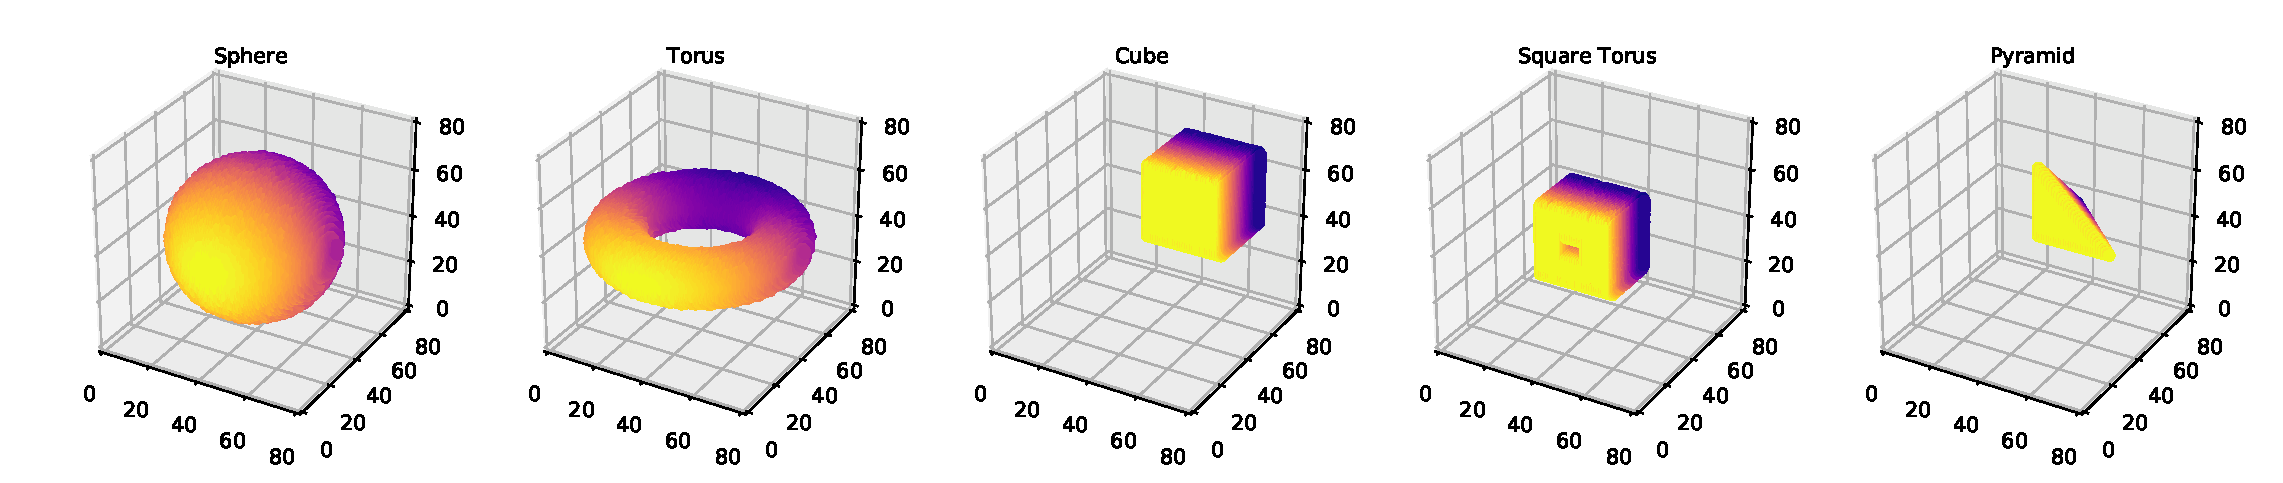
\includegraphics[height=3cm]{graphics/shape_library}}
\caption{A visualization of the various shapes generated. Unless otherwise noted, only spheres and tori were used as a binary decision-making task.}
\label{shape_library}
\end{center}
\vskip -0.2in
\end{figure*}

In our study we will consider only surfaces embedded inside a cube.
For each of these surfaces, there is a method for sampling from its points uniformly randomly - see mathematical preliminaries above.

Since we are doing computations, when we speak of a surface we will mean
implicitly a cloud of points drawn from that surface in a uniform manner.

\subsection{Creating pointcloud data}

Let $S$ be the standard sphere, and $T = T_{r,R}$ the standard torus.

We made $N$ draws of $M$ points from $S$ and $T$ independently and
uniformly - $S_n$ denotes the $nth$ draw of $M$ points from $S$.

Throughout we will call $M$ the sampling rate. We will try $M = 100, 1000,10000$ in our computations.

\subsection{Distortions}

Since humans can identify shapes after they have been distorted or moved around,
we want to see if our neural net will learn to classify the shapes even after these
distorations have been applied. In order to generate data for experiments,
we create random distortions systematically using group theory. These distortions, drawn randomly according to a procedure outlined below, are applied individually
to each training instance as functions on the point clouds generated above. A visualization of
these can be found in Figures \ref{shape_exemplars_to} and \ref{shape_exemplars_sp}.

(To be precise:
An individual experiment works with a fixed collection of distortions $F$, and there is a notion of a random $f \in F$.
We sampled $A_n$ and $B_n$ from $F$ independently and randomly. By $A_n(S_n)$ we mean $A_n$ applied to the sampled pointcloud $S_n$, likewise for $B_n T_n$.
Our pointcloud dataset was $(A_n(S_n), sphere)$ and $(B_n(T_n), torus)$, where $sphere$ and $torus$ were the class labels.)

\begin{figure*}%[ht]
\vskip 0.2in
\begin{center}
\centerline{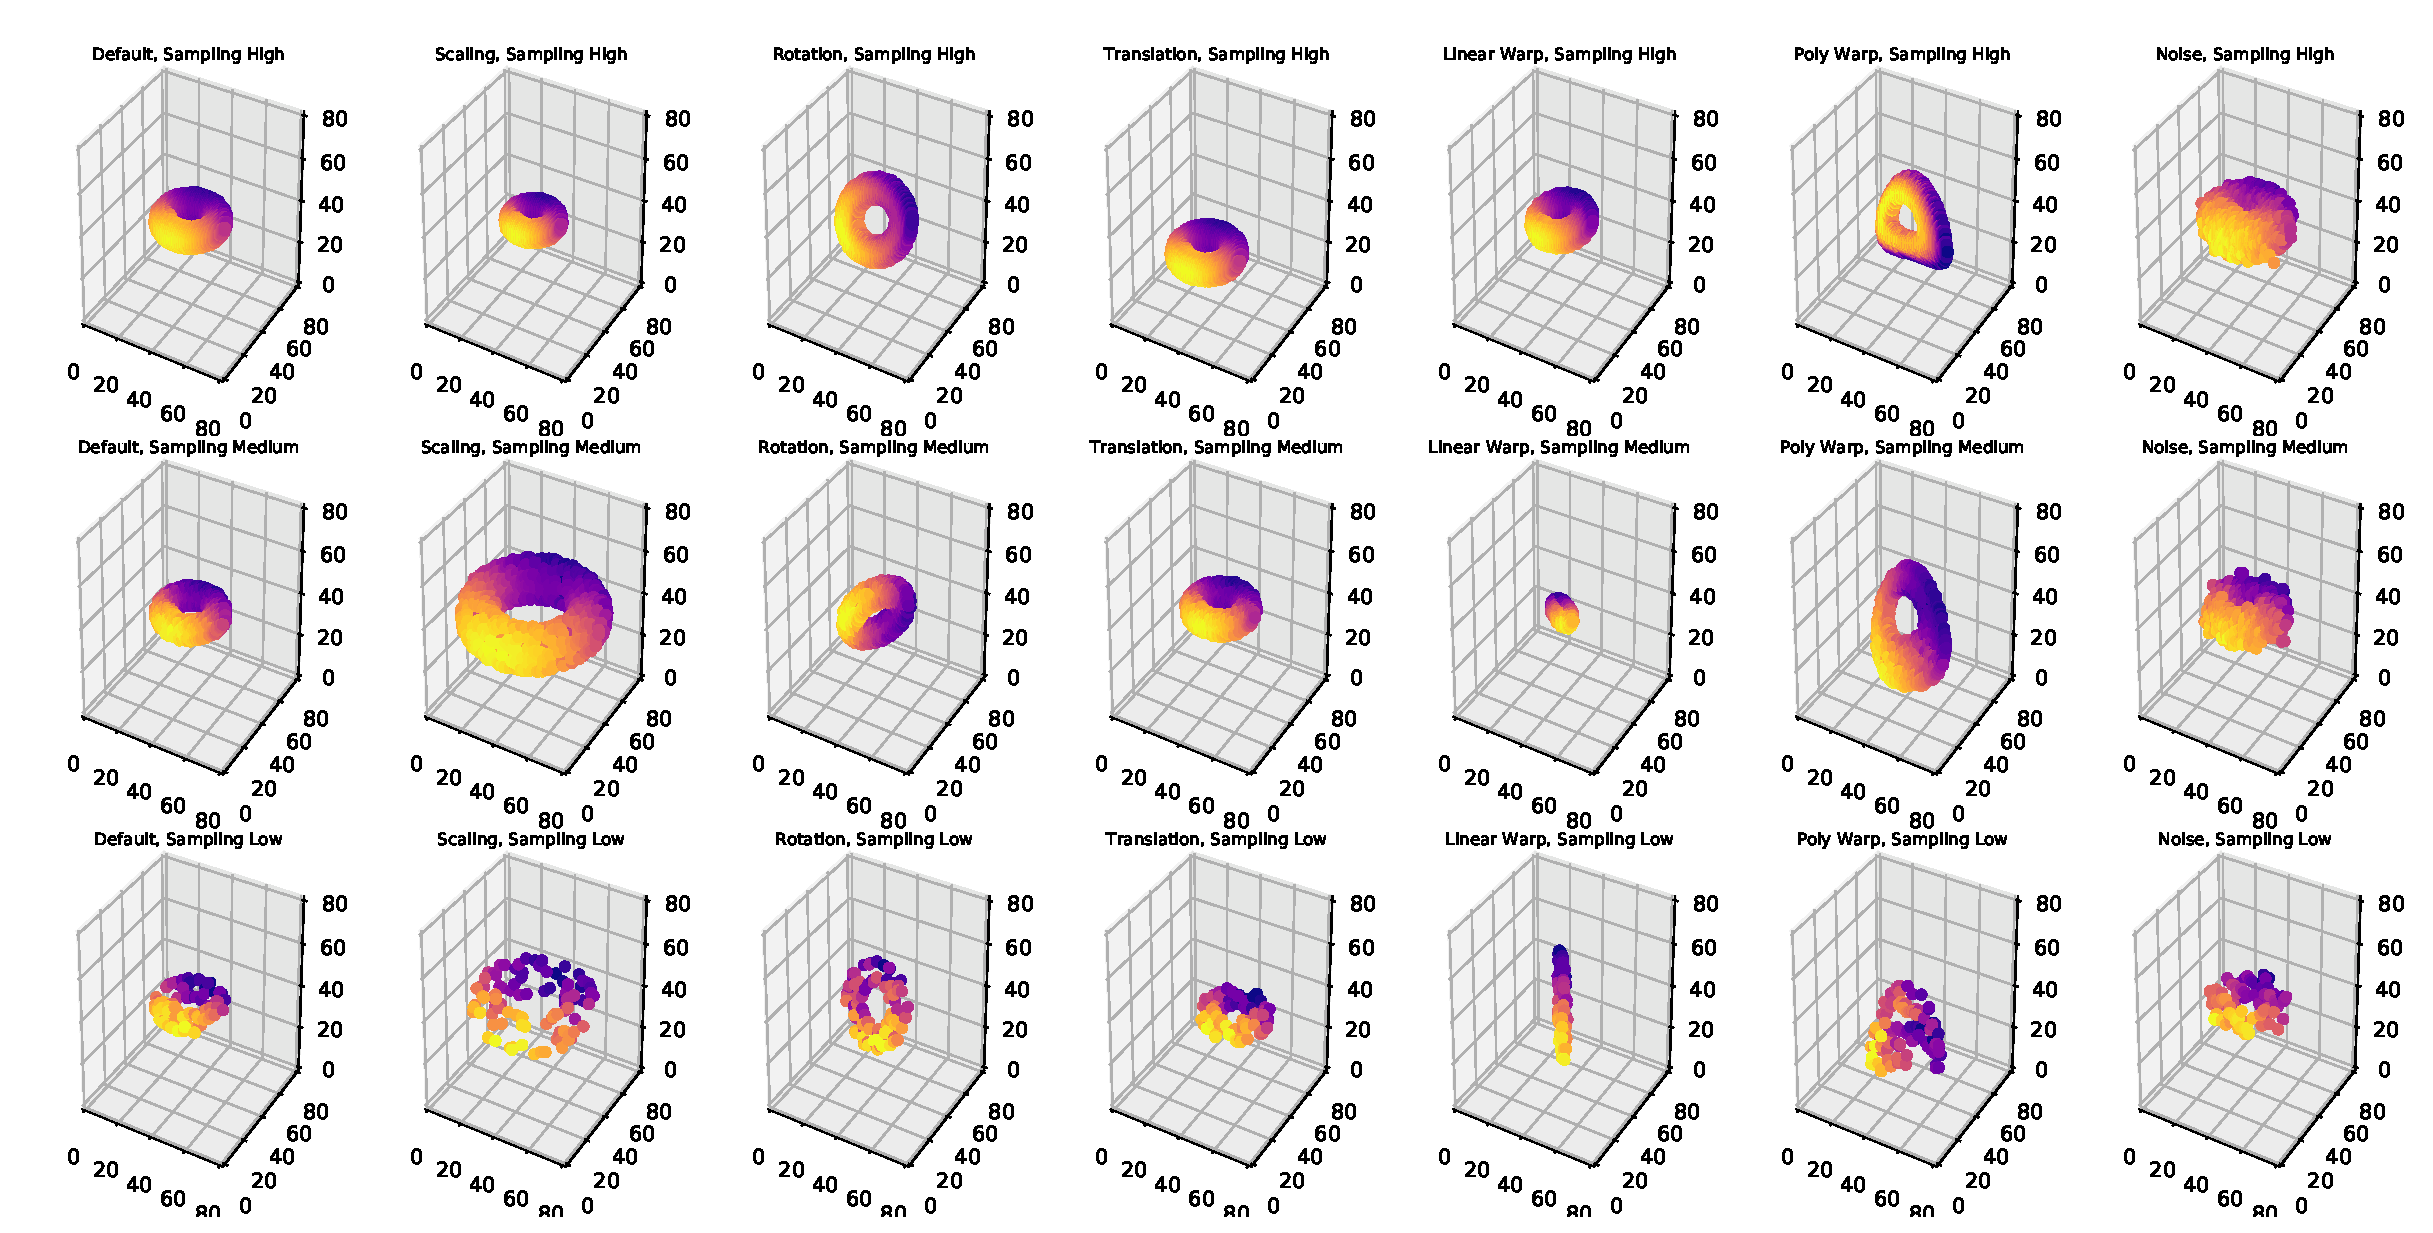
\includegraphics[height=7cm]{graphics/shape_exemplars_to}}
\caption{Examples of toruses with the various distortions applied individually, along with the different sampling frequencies.}
\label{shape_exemplars_to}
\end{center}
\vskip -0.2in
\end{figure*}

\begin{figure*}%[ht]
\vskip 0.2in
\begin{center}
\centerline{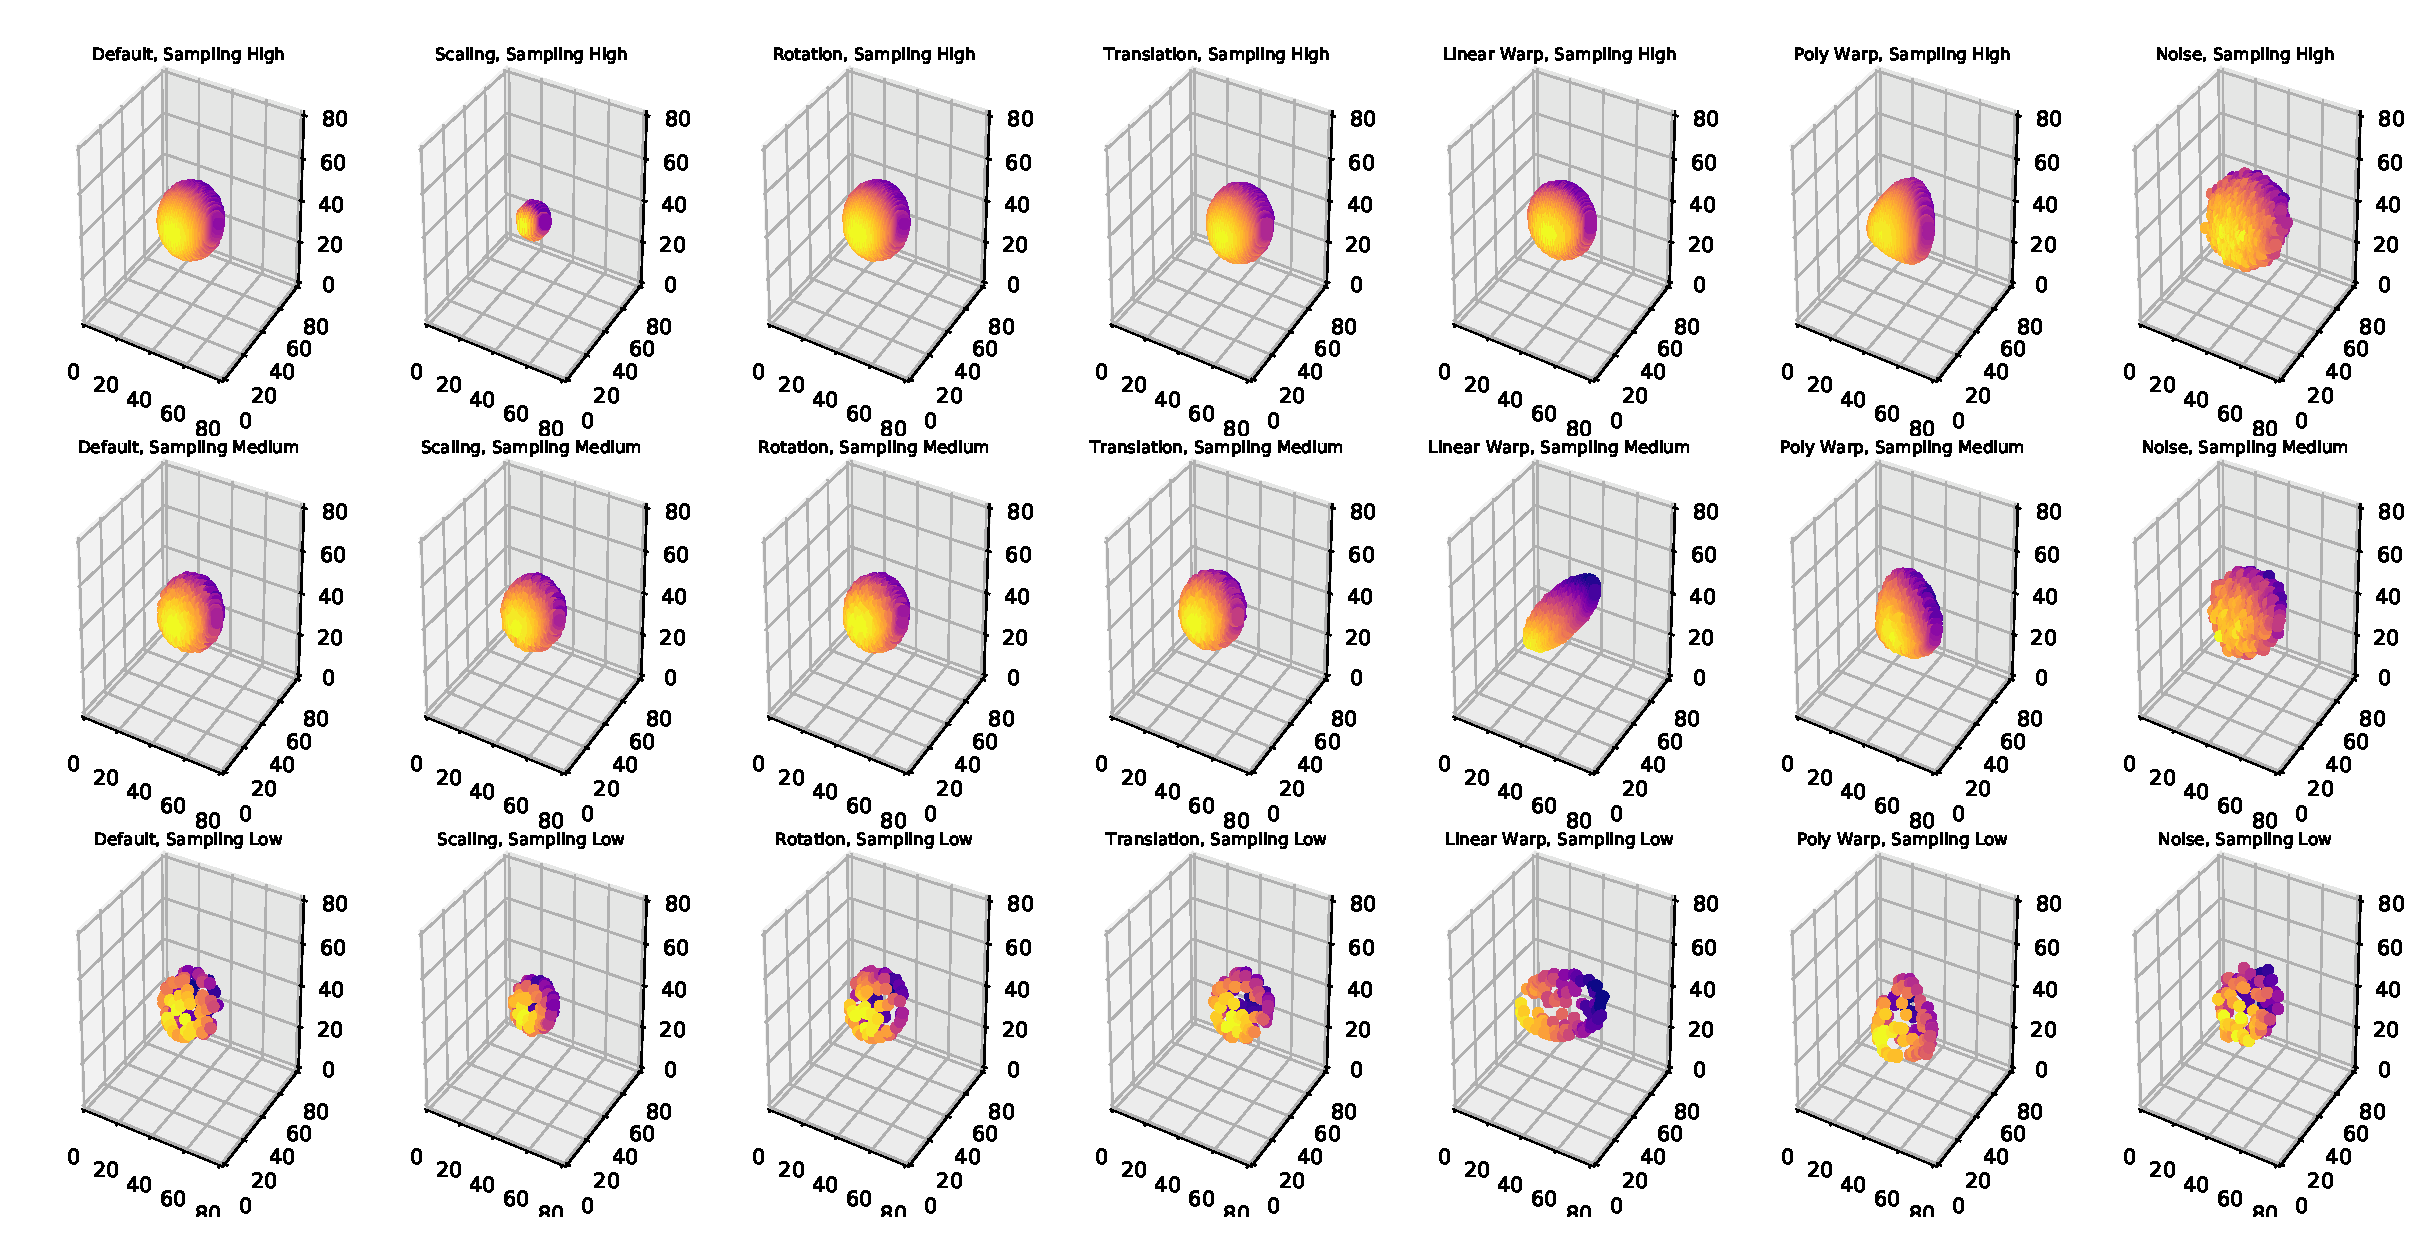
\includegraphics[height=7cm]{graphics/shape_exemplars_sp}}
\caption{Examples of spheres with the various distortions applied individually, along with the different sampling frequencies.}
\label{shape_exemplars_sp}
\end{center}
\vskip -0.2in
\end{figure*}

We used the following kinds of distortions as parameters in our data creation. The input values to generate each distortion are shown in Figure \ref{distortion-settings}

\subsubsection{Default}

A rather uninteresting distortion, this is essentially equivalent to the identity matrix, leaving the original shape intact.
While not particularly interesting itself, it provides a baseline for the other distortions.

\subsubsection{Scaling}

We drew a random scalar in $N(0,\sigma^2)$ to scale our shapes.

\subsubsection{Rotations}

$SO(3)$, the "special orthogonal group," is the collection of rotation matrices in $\mathbb{R}^3$.
Since the composition of two rotations is a rotation, and since the inverse of a rotation is a rotation,
this collection forms a group - an algebraic structure capturing the idea of symmetry.

Group theory assures us that there is a notion of drawing randomly, uniformly from $SO(3)$.
It can be concretely realized by drawing $3$ vectors independently from the standard 3D gaussian,
and performing the Grahm-Schmidt process.

\subsubsection{Translations}

To translate our shapes, we drew a random translation vector from the standard $3D$ Gaussian, with entries drawn from $N(0,\sigma^2)$.

\subsubsection{Linear Warps}

In implementation, we also created the option to draw $A \in SO(3)$ according to the above proceedure
and also add fuzziness to it.This meant that we created a $3x3$ matrix, with entries drawn from a
$N(0, \sigma^2)$, with small $\sigma^2$.

\subsubsection{Polynomial Warps}

Let $p(x,y) = x^2 + y^2$, and let $a > 0$. Define $g_a(x,y,z) = (x,y,z + p(x/a,y/a))$,
and $g_a^{-1}(x,y,z) = (x,y,z - p(x/a,y/a))$. (The polynomial $p$ is not special,
it is just the one that we did experiments with.)

We created another family of distortions by drawing a rotation matrix $A$ randomly
as in the previous subsection, and then applying $g \circ A \circ g^{-1}$ to our shapes.

\subsubsection{Noise}

For each point $x$ in the surface, we made it noisy by adding to it a random
$N(0, \sigma^2)$, with $\sigma^2$ small. The noise was drawn independently for each point.

\subsubsection{All-Except-Polynomial}
This is a compound distortion consisting of scaling, rotation, translation, linear warp, and noise.
Poly was excluded in this set since there is some \textit{a priori} rationale for believing that the
addition of polynomial warps may render it untractable, but without remain tractable. Since we were
interested if this were the case, this compound distortion was included, in addition to \textit{all}.

\subsubsection{All}
This is a compound distortion consisting of scaling, rotation, translation, linear warp,
polynomial warp, and noise. It represents the most complex set of distortions we tested.

\subsubsection{Settings for Each Distortion}
\begin{figure}
\begin{center}
 \begin{tabular}{|c|c|c|}
 \hline
  Distortion  & 2-class Input &  Multi-Class Input   \\ [0.5ex]
 \hline

 Default & none & none\\
 \hline
  Scaling & $\sigma=5$ & $\sigma=3$\\
 \hline
  Rotations & yes/no & yes\\
 \hline
  Translations &  $\sigma=4$& $\sigma=4$\\
 \hline
  Linear Warps & $\sigma=0.3$& $\sigma=0.2$\\
 \hline
  Polynomial Warps & $\sigma=.5$ & $\sigma=0.3$\\

 \hline
  Noise & $\sigma=1$ & $\sigma=1$ \\  [1ex]
 \hline
\end{tabular}
\end{center}
\caption{Input values for each of the nine distortions applied to the shapes.}
\label{distortion-settings}
\end{figure}


\subsection{Preparing data for input to the CNN}

Data used to train the CNN was generated as point clouds in $R^3$ according to the aforementioned methods.
Due to practical constraints, we keep our points on a grid, and limit our region to the unit cube $I^3$.
(There may be fundamentally different approaches... see future directions below for some speculation.)

In particular, we divide our cube up into a grid of small cubes, or ``voxels.''
Each voxel is a feature in the feature vector that serves as input to the CNN.
If a sampled point on the surface of a shape lies in a particular voxel,
then that voxel's input value is non-negative.

We investigated two methods for assigning non-negative input values for features that
correspond to voxels containing one or more points on the surface of a shape.
The first method, our default, is a \textit{binary approach} that assigns a 1
to the features with no points in the corresponding voxel, and a 0 otherwise.
This approach effectively answers the question, ``does this voxel contain a point?''
In contrast, the second method permits features to retain information about how
many points their corresponding voxels contain. In this method, which we term the
\textit{float-based approach}, the input value assigned to feature $i$ is simply
the number of points in voxel $i$ divided by the maximum number of points found
in any given voxel. In other words, for the $i^{th}$ voxel in the set of voxels
$V$, $input_i = \frac{numPoints_i}{max(numPoints_j) \forall j \in V}$.

We hypothesize that the \textit{float-based approach} will lead to higher testing
accuracies in the CNN when noise is present, and sampling is high. This is due to its
ability to encode the extent to which a shape passes through a voxel. For instance,
in Figure \ref{voxel-example} the feature corresponding to the Voxel 1 would have a higher input value than the feature corresponding to Voxel 2.

\begin{figure}
  \centering
      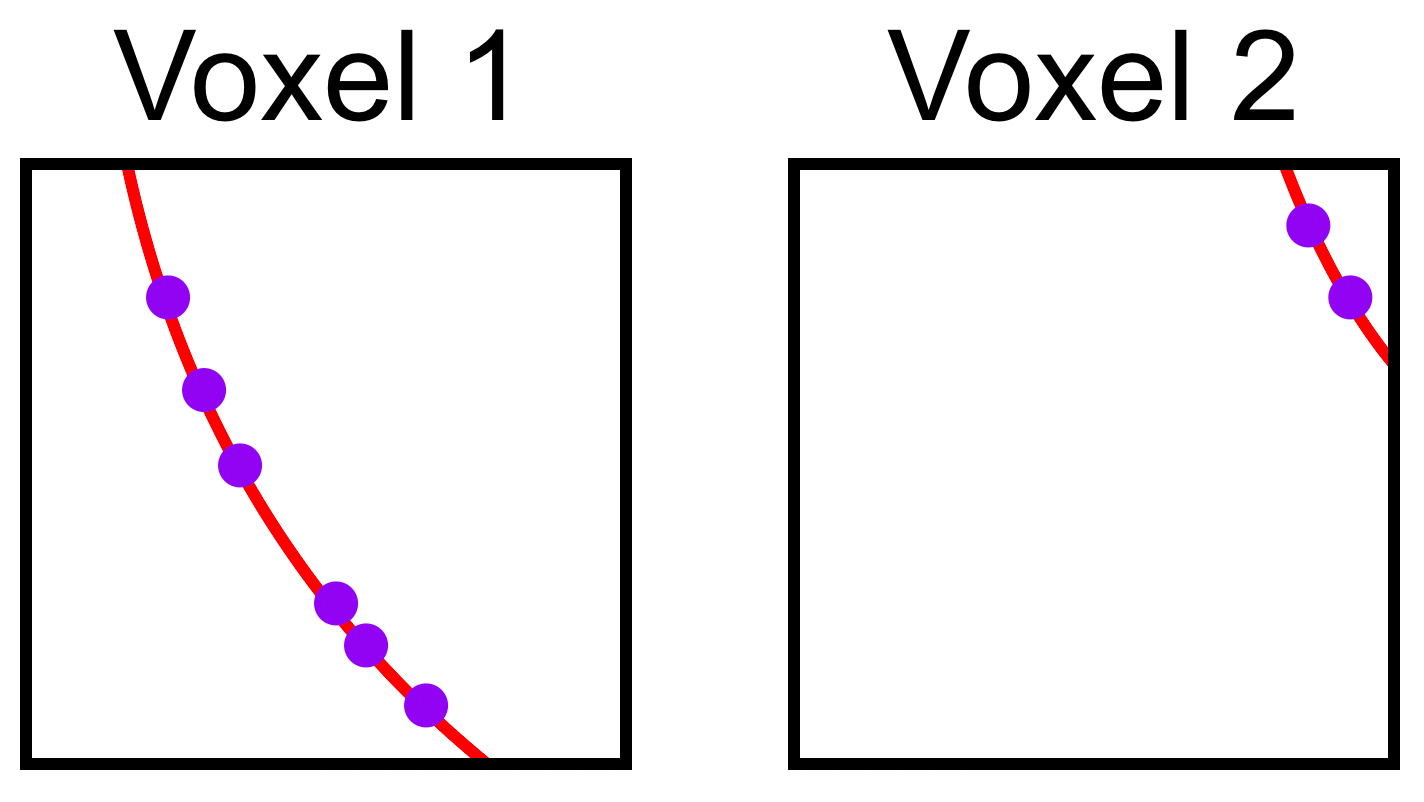
\includegraphics[width=0.3\textwidth]{graphics/float-based-example.png}
    \caption{In this 2D example, the surface of a shape passes more through Voxel 1 than through Voxel 2, resulting in 6 points sampled for Voxel 1 and 2 points sampled for Voxel 2. Using the \textit{float-based approach}, the feature corresponding to Voxel 1 would have $3\times$ the input value as Voxel 2. Using the \textit{binary} approach, both would have input values of 1.}
    \label{voxel-example}
\end{figure}

\subsection{Learning Algorithm}
We trained and tested our data on a 3-dimensional convolutional neural net built using the
Keras deep learning library \cite{chollet2015keras}. The parameters that we used for the
CNN are in Table \ref{CNN_params}, and the structure of the CNN is shown in
Figure \ref{structure}. We varied the number of convolutional layers between 1 and 2,
each with rectified linear unit (ReLU) activation functions, and max-pooled each
convolutional layer with a $2\times2\times2$ pool size. We also added a $20\%$
dropout rate for the convolutional layers. The number of learnable filters was
set to 32 for each convolutional layer, with each filter having a $3\times3\times3$
filter size applied with a stride of $1\times1\times1$. Zero-padding was applied to
each convolutional layer such that the output feature map size was equal to the size of the input.
We also added two fully-connected layers after the convolutional layers, the first with 512 nodes,
and the second with the number of nodes equal to the number of classes in our dataset.
This value is always 2 for our datasets, but can be more in the event that additional
shape-types are classified. For our backpropogation parameters, we used a learning
rate of 0.01 and a momentum of 0.9.  Finally, we trained our CNN with a batch-size of 32.



\begin{table}[t]
\vskip 0.15in
\begin{center}
\begin{small}
\begin{sc}
\begin{tabular}{lcccr}
\hline
\abovespace\belowspace
Parameter & Value \\
\hline
\abovespace
Number of Conv Layers    & 1 or 2 \\
Conv Layer Activation & ReLU\\
Conv Layer Dropout  & 0.2  \\
Number of Filters  & 32   \\
Filter Size  &  $3\times 3\times 3$    \\
Filter Stride      &   $1\times 1\times 1$   \\
Zero-padding  & Yes\\
Pooling Type & Max Pool \\
Pool Size    &.  $2\times 2\times 2$ \\
Learning Rate   & 0.01\\
Momentum    & 0.9\\
Batch Size   & 32\\
\belowspace
\end{tabular}
\end{sc}
\end{small}
\end{center}
\vskip -0.1in
\caption{Summary of CNN parameters}
\label{CNN_params}
\end{table}

\begin{figure}
\begin{center}
 \begin{tabular}{|c|}
 \hline
 Input $80\times80\times80$ grid \\ [0.5ex]
 \hline\hline
 \shortstack{Conv 1: $32\times3\times3\times3$\\ stride: 1, pool: $2\times2\times2$}\\
 \hline\hline
 \cellcolor{gray!25}\shortstack{Conv 2: $32\times3\times3\times3$\\ stride: 1, pool: $2\times2\times2$} \\
 \hline\hline
Fully-connected, 512 nodes \\
 \hline\hline
 Fully-connected, 2 nodes \\
  [1ex]
 \hline
\end{tabular}
\end{center}
\caption{Structure of the CNN. Note that the second convolutional layer, Conv 2, is optional and thus grayed-out.}
\label{structure}
\end{figure}


Finally, we employed an early stopping technique while training our data that resembled the early stopping technique of Lutz Prechelt, which utilizes the error
of the validation set to determine when to stop \yrcite{Prechelt2012}. Specifically,
we stopped when the validation error showed no improvement after 3 epochs. Our primary reason for using early stopping was to take advantage
of when the error of the testing set was likely to be the lowest under the assumption
that the testing and validation set errors would be similar. Other reasons included to prevent
overfitting of the training data, and to decrease the amount of time taken to train.

\subsection{Runtime Environment}
We were unable to run our CNN using UW-Madison's Center for High Throughput Computing. Therefore, training and testing the neural net took place on two personal computers -- one laptop computer running Macintosh OSX with 16 GB of memory and a 2.3 GHz quad core processor, and one desktop computer running Microsoft Windows 7 with 16 GB of memory and a 3.6 GHz quad core processor. Each machine trained and tested separate CNNs, without sharing computing power.

\subsection{Tests}

\subsubsection{Main Analyses}
The main analyses consisted of a 9x3x2 grid, with levels of the aforementioned distortions, sampling rates of $100$, $1000$, and $10000$, and neural nets with
one or two convolutional layers. Accuracies and number of epochs before early stopping were measured for each analysis.

In order to train the net, we split our data into training and testing sets,
with 480 instances initially in the training set and 120 instances in the testing set.
The training set was further split into training and validation sets, with the
final training set having 320 instances and the validation set having 160 instances.
We did not perform k-fold cross validation due to limitations in computing power
available to us. We did not increase the size of the training set for similar reasons.

\subsubsection{Multiclass Analysis}
As a pilot, we also ran an analysis using all 5 shapes and 5-fold cross-validation, and an \textit{all} composition with slightly eased parameters to see if the pattern of errors may
indicate tactics of learning by the Neural Net. Like the main analyses, we split our data into training and testing sets,
with 480 instances initially in the training set and 120 instances in the testing set.
The training set was further split into training and validation sets, with the
final training set having 320 instances and the validation set having 160 instances.
To gauge the importance of training size in this domain, we also ran another test with double the training size,
validation size, and testing size.
Unlike the main analyses, all tests were done with the floating-point method of sampling, with a sampling rate of 10000.


\section{Results}
In order to discriminate the difference between input shape variation parameters and
the capabilities of a CNN to learn them, we have separated our analyses into two major
categories: Parameters, and Limitations and Capabilities.

Parameters refers to the different types of variations we can impose on the input data,
such the types of shapes drawn from and the
distortions which distinguish different instances, such as translation,
rotation, etc. (see section 3.3). We also investigate the effect of different sampling rates on the shape surfaces on a logarithmic scaling from sampling 100 points (low) to 1000 points (medium), to 10000 points (high). All of the aforementioned parameters are varied with one and two convolutional layers using the \textit{binary approach} for assigning input values to features corresponding to voxels. Finally, we performed four additional experiments which used the \textit{float-based approach} of assigning input values to features corresponding to specific voxels. The experiments were performed with \textit{translation}, \textit{linear warp}, \textit{all (except poly)}, and \textit{all} parameter settings with a sampling rate of 10000 and one convolutional layer.

Regarding limitations and capabilities, we investigate the effect of the different parameters and input data on the CNN.

\begin{table*}[t]
\vskip 0.15in
\begin{center}
\begin{small}
\begin{sc}
\begin{tabular}{lcc|cc|cccr}
\hline
\abovespace\belowspace
Parameter Tests         & \multicolumn{2}{c}{Sampling 100 (Low)} & \multicolumn{2}{c}{Sampling 1000 (Medium)} & \multicolumn{4}{c}{Sampling 10000 (High)} \\
\hline
                        & Accuracy  & Epochs   & Accuracy  & Epochs   & Accuracy  & Epochs   & Accuracy  & Epochs\\
\hline
\abovespace
Default                 & $100\%$   & $23$     & $100\%$    & $5$    & $100\%$   & $5$  &                            & \\
Scaling                 & $87.5\%$  & $6$      & $100\%$    & $25$   & $100\%$   & $12$ &                            &   \\
Rotation                & $49.17\%$ & $5$      & $100\%$    & $5$    & $100\%$   & $5$  &                            &  \\
Translation             & $50\%$    & $10$     & $93.33\%$  & $10$   & $92.5\%$  & $6$  & \textcolor{blue}{$97.5\%$} & \textcolor{blue}{$12$}       \\
Linear Warp             & $46.67\%$ & $5$      & $95.83\%$  & $8$    & $95\%$    & $8$  & \textcolor{blue}{$95\%$}   & \textcolor{blue}{$8$}             \\
Poly Warp               & $52.5\%$  & $10$     & $100\%$    & $6$    & $100\%$   & $5$  &                            &  \\
Noise                   & $100\%$   & $25$     & $100\%$    & $6$    & $100\%$   & $5$  &                            & \\
All (Except Poly)       & $54.17\%$ & $5$      & $45\%$     & $7$    & $43.33\%$ & $9$  & \textcolor{blue}{$52.5\%$} & \textcolor{blue}{$5$}            \\
All                     & $48.33\%$ & $13$     & $100\%$    & $5$    & $58.33\%$ & $7$  & \textcolor{blue}{$55\%$}   & \textcolor{blue}{$5$}           \\
\end{tabular}
\end{sc}
\end{small}
\end{center}
\vskip -0.1in
\caption{A description of the different parameters and results for a neural net with a single convolutional layer. \textcolor{blue}{Results in blue indicate a float-based approach.}}
\label{table:results1}
\end{table*}

\begin{table*}[t]
\vskip 0.15in
\begin{center}
\begin{small}
\begin{sc}
\begin{tabular}{lcc|cc|cccr}
\hline
\abovespace\belowspace
Parameter Tests         & \multicolumn{2}{c}{Sampling 100 (Low)} & \multicolumn{2}{c}{Sampling 1000 (Medium)} & \multicolumn{4}{c}{Sampling 10000 (High)} \\
\hline
                        & Accuracy  & Epochs   & Accuracy  & Epochs   & Accuracy  & Epochs   & Accuracy  & Epochs\\
\hline
\abovespace
Default                 & $100\%$   & $25$     & $100\%$    & $5$    & $100\%$   & $5$  &    & \\
Scaling                 & $50.8\%$  & $5$      & $99.17\%$  & $15$   & $48.33\%$ & $5$  &    & \\
Rotation                & $49.17\%$ & $5$      & $100\%$    & $8$    & $100\%$   & $6$  &    & \\
Translation             & $50.83\%$ & $6$      & $90\%$     & $7$    & $95.83\%$ & $15$ &    & \\
Linear Warp             & $52.5\%$  & $5$      & $50\%$     & $7$    & $97.5\%$  & $19$ &    & \\
Poly Warp               & $53.33\%$ & $5$      & $100\%$    & $12$   & $100\%$   & $25$ &    & \\
Noise                   & $100\%$   & $23$     & $100\%$    & $6$    & $100\%$   & $5$  &    & \\
All (Except Poly)       & $55.83\%$ & $7$      & $50.8\%$   & $6$    & $52.5\%$  & $6$  &    & \\
All                     & $55\%$    & $6$      & $54.17\%$  & $5$    & $51.67\%$ & $10$ &    & \\
\end{tabular}
\end{sc}
\end{small}
\end{center}
\vskip -0.1in
\caption{A description of the different parameters and results for a neural net with two convolutional layers. \textcolor{blue}{No tests were run with a float-based approach.}}
\label{table:results2}
\end{table*}

\subsection{Parameters}

\begin{figure}
  \centering
      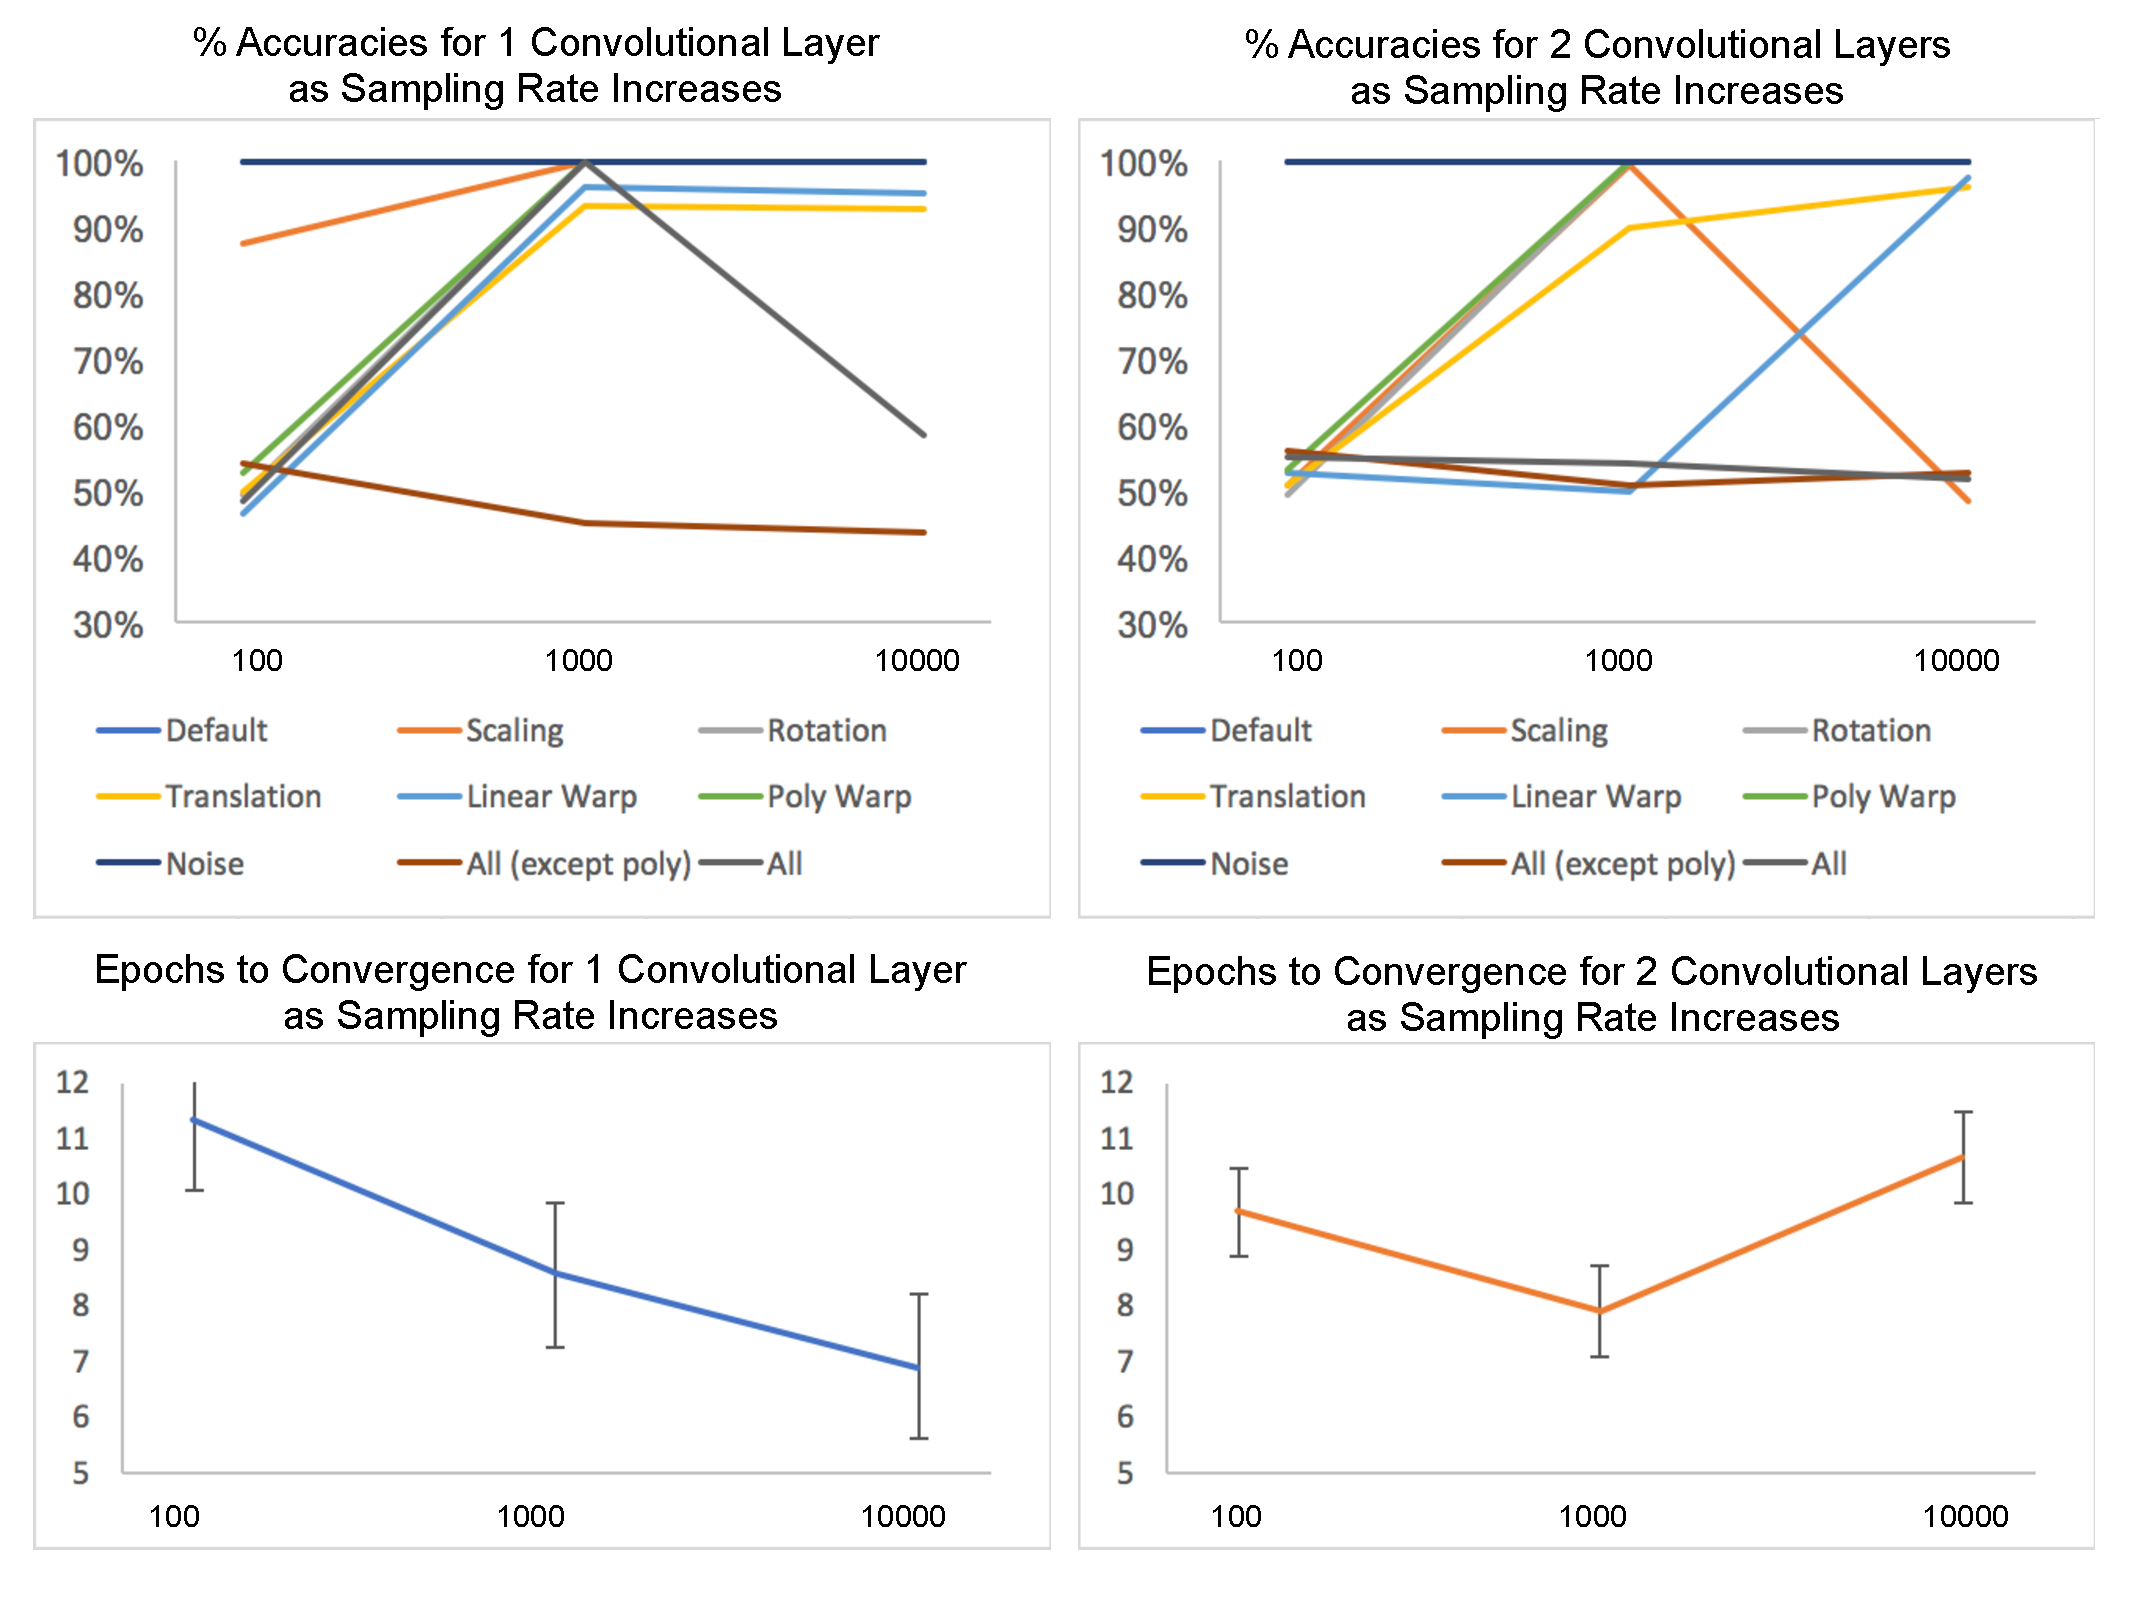
\includegraphics[width=0.5\textwidth]{graphics/results_graphs2.pdf}
    \caption{Testing accuracy plotted against sampling rate \textit{(top)}, and time-to-convergence plotted against sampling rate $bottom$.}
    \label{results-graph}
\end{figure}

Our results for each parameter setting are shown in Tables \ref{table:results1} and \ref{table:results2}. Each table is a $9\times3$ parameter grid of tests for either one or two convolutional layers. These results contain both the $\%$ accuracy for each dataset and number of epochs taken to converge in these settings. The percent-accuracy results are summarized in Figure \ref{results-graph}, which show the behavior of the testing accuracies as the number of points sampled increases.

Figure \ref{results-graph} indicates that for CNNs with 1 convolutional layer, the testing accuracy increases for most parameter settings as the sampling rate increases. This finding does not hold when the \textit{all} and \textit{all (except poly)} distortions are applied. With \textit{all}, the testing accuracy increases going from $100$ samples to $1000$ samples, but decreases with $10000$ samples. This decrease may be due to the low number of instances used for training, and the fact that we did not train with k-fold cross validation. With \textit{all (except poly)}, the testing accuracy when all dataset parameters are varied steadily decreases as the sampling rate increases. The accuracy results for 2 convolutional layers are more mixed. The accuracies for \textit{all} and \textit{all (except poly)} show little to no change at all. Additionally, the testing accuracy for \textit{scaling} increases going from $100$ samples to $1000$ samples, but decreases with $10000$ samples. Again, this decrease of accuracy may be a result of both the low number of instances used for training, and the fact that we did not apply k-fold cross validation.

Additionally, Figure \ref{results-graph} shows the effect on the number of epochs taken to converge as the sampling rate increases. The number of epochs taken to converge was calculated as the minimum of when early stopping occurred and 25 epochs. 25 epochs was the maximum number of epochs in which training could occur. On average, for both one and two convolutional layers, increasing the sampling rate decreases the time to convergence.

Lastly, Figure \ref{results-graph} shows that for the four experiments performed with the \textit{float-based approach}, there was no significant difference in resulting testing accuracy. We thus performed no further trials with the \textit{float-based approach}.

\subsection{Capabilities and Limitations}
We would expect the accuracy of the CNN on a testing set to increase as the sampling rate increases, since higher sampling rates lend to more accurate shape representations in voxel space. This is indeed the case in our results, minus a few instances where the accuracy was stagnant across sampling rates, and a few instances in which the accuracy increased briefly for $1000$ samples, but decreased again for $10000$. Suppose we attribute the latter to our small training sets and the fact that we did not employ k-fold cross validation in training the net. In other words, periodic poor performance of the net caused by our low training set size is not mitigated by higher performance of other folds. Then, it is indeed the case that higher sampling rates lead to more accurate classification of shapes. Therefore, the following discussion of the capabilities and limitations of the net will be limited to the experiments with a sampling rate of 10000 points.

From Table \ref{table:results1}, it is clear that the CNNs which were trained and tested by varying zero or one shape distortion, such as \textit{default}, \textit{rotation}, or \textit{scaling}, performed better than
the \textit{all} and \textit{all (except poly)} parameter settings. This is also evident in the ROC curves for the experiments. Figure \ref{ROCgraph} shows two example ROC curves, one from the \textit{translation} shape distortion and the other from the \textit{all (except poly)} shape distortion sampled at 10000 points in a CNN with a single convolutional layer. These two results are chosen for analysis due to their being representative of distortions that the CNN learned well and not so well.

\begin{figure}
  \centering
      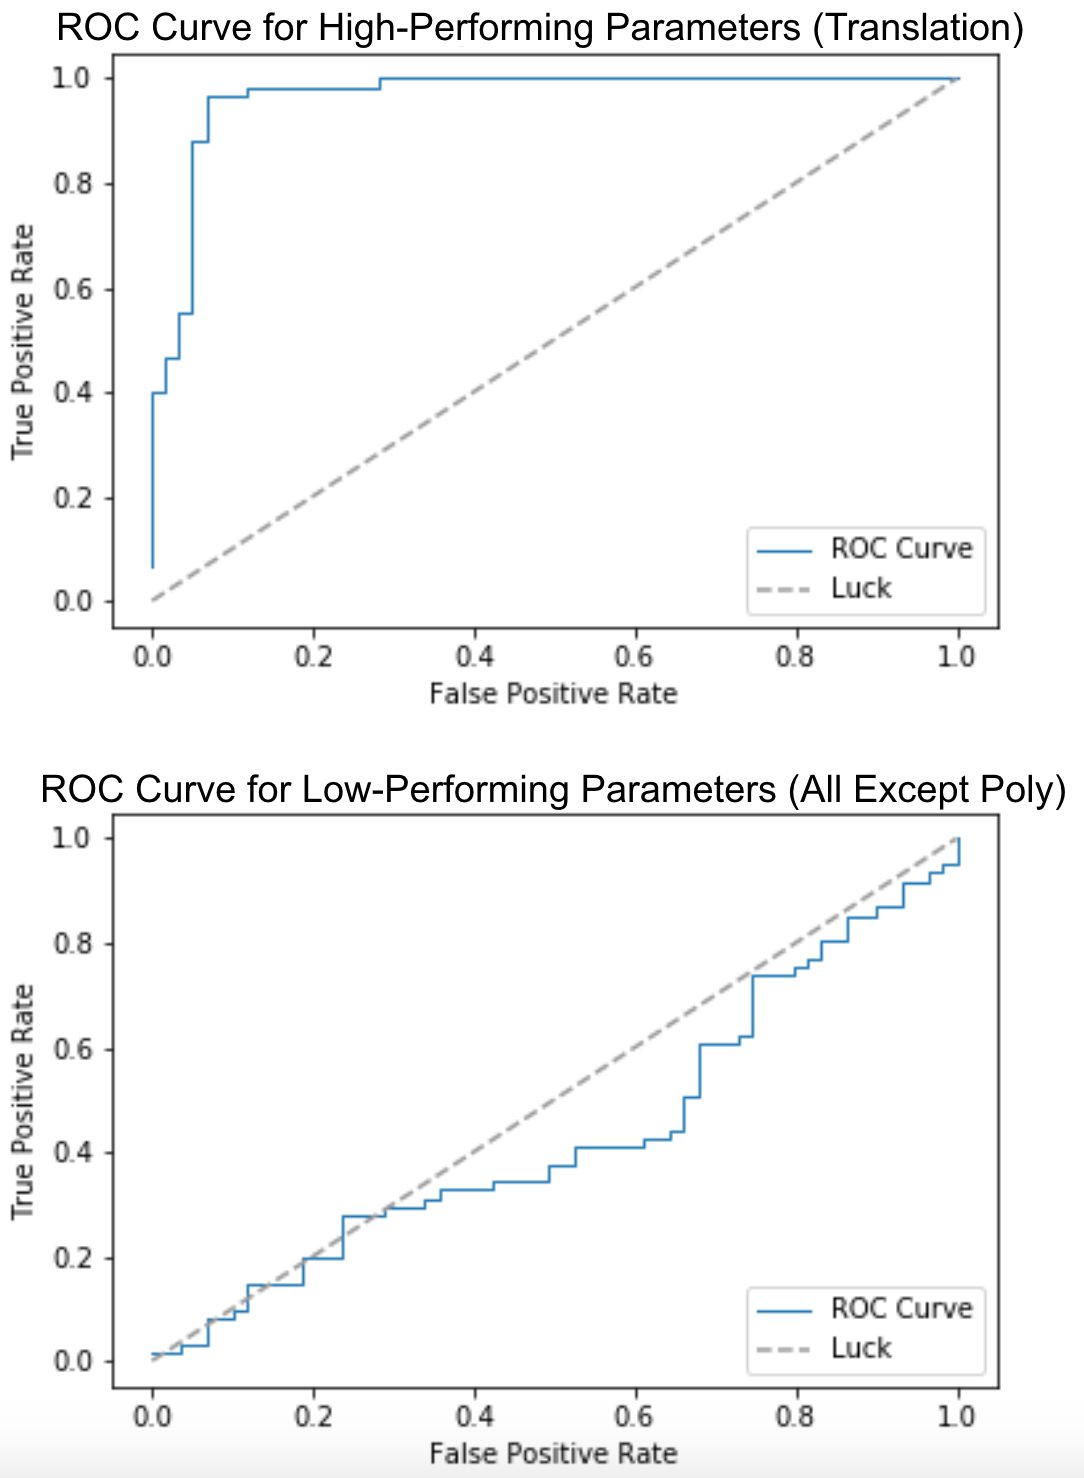
\includegraphics[width=0.5\textwidth]{graphics/roc.png}
    \caption{ROC curves for both a high and low-performing parameter settings.}
    \label{ROCgraph}
\end{figure}

\begin{figure}
\begin{center}
 \begin{tabular}{|c|c|c|}
 \hline
  & Torus True  & Sphere True \\ [0.5ex]
 \hline
 Torus Prediction & 28 & 27 \\
 \hline
 Sphere Prediction & 31 & 34 \\ [1ex]
 \hline
\end{tabular}
\end{center}
\caption{Confusion matrix for \textit{all (except poly)} with a sampling rate of 10000 and a single convolutional layer}
\label{confusion-binary-bad}
\end{figure}

\begin{figure}
\begin{center}
 \begin{tabular}{|c|c|c|}
 \hline
  & Torus True & Sphere True \\ [0.5ex]
 \hline
 Torus Prediction & 56 & 5 \\
 \hline
 Sphere Prediction & 4 & 55 \\ [1ex]
 \hline
\end{tabular}
\end{center}
\caption{Confusion matrix for \textit{translation} with a sampling rate of 10000 and a single convolutional layer.}
\label{confusion-binary-good}
\end{figure}

The ROC curve for \textit{all (except poly)} clearly shows that the CNN is performing worse than chance. For most given false positive rates, the true positive rate is worse. Contrastingly, the ROC curve for \textit{translation} shows a high true positive rate for most given false positive rates. The confusion matrices for both sets of parameters tells a similar story. For \textit{all (except poly)}, the confusion matrix shows that each shape is more often being classified incorrectly than correctly, whereas the confusion matrix for \textit{translation} shows shapes being overwhelmingly classified correctly.

Additionally, the CNN overfit to the training set in the experiments with low testing set accuracies. In \textit{all (except poly)}, for instance, the training set accuracy at early stopping was $97.81\%$, whereas the testing set accuracy was $43.33\%$. Similar discrepancies in training and testing sets are found for all other results with low testing set accuracies.

There is not much difference in all aspects of the results between the experiments with one or two convolutional layers. However, the experiments with two convolutional layers did take longer to converge than the experiments with one convolutional layer, in general (Figure \ref{results-graph}). Similar to varying the number of convolutional layers, the few experiments that varied the \textit{binary approac} and \textit{float-based approach} to assigning non-negative input values to the CNN showed no significant difference in testing accuracies.

The above results indicate that in general, our method for training CNNs to classify 3-dimensional shapes is strong when classifying shapes that have undergone no distortions, or a single distortion so long as all shapes have undergone the same distortion in some way. However, our method falls short when classifying shapes that have undergone a composite of distortions, to the point that classification is no better than or worse than chance. Additionally, changing the number of convolutional layers from 1 to 2 results in no discernible difference in testing set accuracies.

\subsection{Multiclass Analysis}

\begin{table*}[t]
\vskip 0.15in
\begin{center}
\begin{small}
\begin{sc}
\begin{tabular}{lcc|ccr}
\hline
\abovespace\belowspace
Parameter Tests         & \multicolumn{2}{c}{Standard Training Size} & \multicolumn{2}{c}{Double Training Size}\\
\hline
                        & Accuracy  & Epochs   & Accuracy  & Epochs \\
\hline
\abovespace
Fold 1                  & $32.5\%$  & $6$      & $33.33\%$  & $7$    \\
Fold 2                  & $21.67\%$ & $6$      & $38.75\%$  & $6$   \\
Fold 3                  & $31.67\%$ & $5$      & $32.5\%$   & $5$    \\
Fold 4                  & $29.17\%$ & $5$      & $35\%$     & $6$    \\
Fold 5                  & $20.83\%$ & $5$      & $20\%$     & $5$    \\
\end{tabular}
\end{sc}
\end{small}
\end{center}
\vskip -0.1in
\caption{Accuracy and epochs before early stopping for standard training size and double training size runs.}
\label{multiclass_results}
\end{table*}

Results from two 5-fold cross-validation runs on the multi-class discrimination task are shown in
Table \ref{multiclass_results}. In general, accuracies ranged from chance, 20\% to 38\%. Number of epochs before early stopping ranged from 5 to 7.

Training accuracy usually rose fast, despite the low test accuracy - sometimes as high as 80\%.
This coincided with an increasing validation error, causing the early stopping to engage.
These two facts mean that overfitting was likely occurring.

\begin{figure*}
\begin{center}
    \begin{tabular}{|c|c|c|c|c|c|}
    \hline
    &Torus & Pyramid & Cube & Sphere & Square Torus \\ [0.5ex]
    \hline
    \shortstack{Torus \\Prediction}        & $14$  & $6$     & $8$  & $15$   & $1$  \\
    \hline
    \shortstack{Pyramid \\Prediction}     & $4$   & $23$    & $9$  & $8$    & $16$ \\
    \hline
    \shortstack{Cube \\Prediction}        & $7$   & $4$     & $11$ & $6$    & $8$  \\
    \hline
    \shortstack{Sphere \\Prediction}       & $15$  & $2$     & $1$  & $14$   & $3$  \\
    \hline
    \shortstack{Square Torus \\Prediction} & $7$   & $17$    & $19$ & $6$    & $16$ \\ [1ex]
    \hline
   \end{tabular}
\end{center}
\caption{A confusion matrix for the 5-class discrimination task.}
\label{multiclassconfusion}
\end{figure*}

As can be seen in Figure \ref{multiclassconfusion}, an example confusion matrix from the \textit{double-training-size} test is presented.
From this matrix, it appears that the CNN is having difficulty distinguishing between smooth shapes (spheres and tori), and "edged" shapes (cubes, pyramids, and square tori)
This specific example seems to indicate the presence of corners may be important.

\section{Discussion}

\subsection{Efficacy}

The neural net was mostly successful at learning the binary classification problems it faced when the distortions were non-composite.
As mentioned before, increasing the sampling rate usually has the effect of improving accuracy. Interestingly, adding a second convolutional
layer has a negligible if not detrimental effect on the neural net's efficacy.

The attempt of classifying between 5 different shapes was not as successful, achieving slightly better than chance.
It is still impressive, given the algorithm was performing a quinternary discrimination task on a slightly easier
version of parameters for a composite distortion that was effectively intractable for the binary discrimination task.
Due to time constraints we were unable to study whether ensemble methods such as
error-correcting codes \cite{dietterich1995solving}
could improve efficacy for the binary or quinternary discrimination tasks,
but this is a clear future avenue of testing.

\subsection{Thoughts on PAC Learnability}

Based on our computational results, we make the following (vague) conjecture:

Conjecture: Let $G$ be a (compact) group of transformations of $\mathbb{R}^3$.
Let $S$ and $T$ be surfaces. Then the problem of distinguishing $gS$ and $g'T$ for
uniformly random $g,g' \in G$ is (PAC) learnable by a (convolutional) neural network,
provided there is no $g \in G$ so that $gS$ and $T$ are ``very similar''.

Compactness is a technical assumption that limits the ``size'' of the space of transformations. This includes $SO(3)$.

To be precise, our instance space is the space of $n$ points $\mathbb{R}^3$, for $n$ very large. This is called the configuration space of points in space, and is a very well studied object.
For a surface $S$, the concept $c_S$ is the set of $n$ points that together
lie on some from $gS$, for some $g \in G$, with notation as in the conjecture.
The concept class $C$ is the set of $c_X$, for $X \in \{S,T\}$.

In our experiment we drew samples by
picking $g$ randomly, and drew from $gS$ uniformly, or from $gT$ uniformly,
and labelling as $1$ or $0$. General PAC learning would require drawing from an arbitrary distribution.

We claim that if $\epsilon, delta > 0$, there
is a polynomial $p$ in $1/\epsilon$ and $1 / \delta$ (and possible other parameters, such as the dimension or complexity of $G$) so that we need $p$ samples
in order to produce, with probability $1 - \delta$ a neural net that has average error
less than $\epsilon$.

Making further progress on this conjecture would require further study of neural net outside the scope of this paper.

\subsection{Mathematical Shape Classification - Isomorphism and invariants - What is our network learning?}

Human mathematicians have developed two key concepts for classifying shapes. The first idea is a hierarchy of thresholds for equivalences of shapes under some specified type of distortions; each level of the hierarchy is called a category. For example, two spheres $A$ and $B$ in 3-space with $radius(A) = 1$, $radius(B) = 2$ will be equivalent if we allow scaling and translations (working in ``the category of spheres in 3-space with translations and scalings''), but not so if we only allow translations (working in ``the category of spheres in 3-space with translations'').  An equivalence is ``witnessed'' by a function of the allowed type, and this witness is called an isomorphism -- in the example with spheres, the witness function would be the translation and scaling of 3-space that moves $A$ onto $B$.

In general, given two shapes $A$ and $B$, it may be valuable to prove or disprove that they are equivalent in some interesting category. Unfortunately, there are often many candidate distortions that could witness an equivalence of $A$ and $B$, and it is impractical to check each one. This leads to the second key idea, which is the notion of invariant - in the examples above, we could see that sphere $A$ is not equivalent to sphere $B$ under $\{Translations\}$, because the radius doesn't change when we translate, and the radii of $A$ and $B$ are different. In this case, the radius of the sphere is an invariant of the equivalence relationship described by translations. Thus we say that the radius is a $\{Translations\}$-invariant, or is translation invariant.

In general, for any notion of equivalence, a primary strategy for showing that two shapes differ is to produce an invariant for that equivalence that the shapes differ on, especially when the space of candidate distortions between the shapes is too large to search through and exhaustively demonstrate the non-existence of a witness to equivalence.

Suppose we have two shapes $A$ and $B$ in 3-space, and some collection of distortions $F$, and suppose that there is some $F$-invariant of $A$ and $B$, $I(A) \not = I(B)$. We feed a neural net the data: $fA$ labeled with $A$ and $fB$ labeled with $B$ for many random $f \in F$. If we hand our neural net some $f'A$ or $f'B$ and it correctly classifies it as $A$ or $B$, we will say that the neural net has become $F$ invariant. It is implausible that it checks every possible candidate witness, so we can wonder if it has has it learned to compute $I$, or some other invariant of $F$?

One way to gain some insight into this question is to change $F$ to be a different set of distortions $G$, and see if the network is also $G$ invariant. We can do this systematically by choosing a direction $v$ to deform the transformation in, and see if the network remains $H_{t,v}$ invariant, for small $t$. (For example, choose a  $1$ parameter subgroup of $Diff(\mathbb{R}^3)$  $\phi(t)$, and use $H_{\phi, t} = \phi(t) \text{AffineGroup}(3) \phi(t)^{-1}$. We have to learn more about $Diff(\mathbb{R}^3)$.) We could also use this idea to produce a neural net which is more robust to changes in $F$, by picking many directions and building a training set using their transformations. We have started to study this question , but haven't had time to finish the computations.

Note that the idea of an invariants is for us really probabilistic:Let $I$ be some candidate computation from shapes to real numbers. Then it is possible that the distribution of $I(fA)$ for random $f \in F$ is far from the distribution of $I(fB)$ for random $f \in F$ (say in KL-divergence), but has some overlap. In this case, we may only be able to say that a mystery object is $fA$ for some $f \in F$ with some probability, and $f'B$ for some $f' \in F$ with some other probability. (For example, if $A$ is a big sphere, and $B$ is a small sphere, then $I$ could be average distance from the origin, and random $F$ given by translation vectors drawn from a Gaussian distribution.) It is reasonable that our network has learned something along these lines, since it learns a probabilistic classifier.

We wonder if the invariants mathematicians have discovered to be useful are somehow implicit in the structure of a neural net, or if these sort of investigations could lead to useful new invariants for mathematicians to investigate. We didn't have time to computationally investigate this question sufficiently. However, our code is set up to do this, and we plan to continue to play with parameters.

\subsection{Future Directions, Speculations and Open (to us) Questions}

\subsubsection{Parameters for CNNs}
Due to compute time restrictions, we were unable to test a full array of parameters.
Future work could look at increasing the dataset size, employing k-fold cross validation and tiling, and tweaking various CNN parameters. For the dataset size, we were restricted by the processing and memory requirements of our personal computers. We would therefore like to increase the number of instances used in the training and testing sets in conjunction with k-fold cross validation to increase the accuracy of the testing results. For pre-processing of the data, we would like to look into pre-processing the input data and tiling the CNN as a way to allow the net to learn different invariances \cite{Le10tiledconvolutional}. Lastly, the approach investigated in this work focused mainly on varying parameters of the input data, rather than parameters of the CNN. Therefore, as a next step we would like to vary parameters of the net, starting with parameters that combat overfitting, such as dropout and pooling.

\subsubsection{Storing shapes and moduli spaces}

What is the right data type for teaching a computer about a shape?
If we sample from a shape, what is the right way to store the pointcloud? Mathematically, we are satisfied with a set of points, but storing a set in a computer puts an ordering on the points, and the unnatural order contributes to noise.
Our solution to this question was to store the shapes as a non-negative function on voxels.

We could phrase our algorithm as this diagram: $\{\text{Pointcloud}\} \\ \downarrow_{\text{Estimator}} \\ M = \{\text{functions on voxels}\} \\ \downarrow_{\text{Neural Net}} \\ \{\text{Class of shape}\}$.

While we experimented with changing the estimator, it is plausible that we could experiment with $M$ as well, and put in its place a space that is tailored to the geometric problem at hand. For example, if we were studying shapes cut out by quadratic algebraic equations in $x,y,z$, then we could investigate an maximum likelihood estimator onto the space of coefficients of quadratic equations in $x,y,z$ - this is $\mathbb{R}^N$ with coordinates $a_{ij}$ corresponding to the general quadratic equation $\Sigma_{i + j \leq 2} a_{ij}x^iy^j = 0$. The neural net would then take as input the coefficients of the quadratic equations, rather than the function on voxels. Such candidate spaces $M$ are heavily studied in modern geometry, under the names parameter space and moduli space.

\subsubsection{Symnets and Curvature invariants}

If an ant wanders forever on a surface, then by keeping track of how the landscape
curves around it, it will be able to compute whether it lives on a sphere or torus. This is a special case of the Gauss-Bonnet theorem.
Mathematically, this is expressed as an integral over the surface of a measurement
of the curving of the surface, called Gaussian curvature. The average amount of curving classifies a shape as either a sphere or a torus.

For any point on the unit sphere, the Gaussian curvature will be one -- even though from the point of view of CNN, which allow
only translational symmetries, the various regions of the sphere look different. However,
if we allowed the feature window to rotate, it could recognize that each of these regions was
fundamentally the same, and exploit that.

If we used a NN architecture that allowed for different transformations of the feature window,
it's plausible that the machine could learn an approximation to Gaussian curvature on
little patches of a surface, and average them to classify the shape as a torus or sphere.

Symnets \cite{symnets} are an approach to this problem that uses the entire affine group rather than just the translation group
to build a neural net. We did not have time to explore this direction, but this is a potential avenue of future computational experimentation.

\subsubsection{Persistent homology}

Topological data analysis is a field of mathematics that concerns itself with building algorithms
to detect the topology of pointclouds; their methods (in principle) accurately solve the classification problem we posed here. We wonder about a comparison of highly trained neural net with their algorithms.

\subsubsection{Generative Adversarial Networks}

In the interest of further desciphering the feature learning of neural networks in the
shape domain, a clear future direciton is the area of Generative Adversarial Networks
(GANs) \cite{goodfellow2016nips}. By employing a game-theory tactic of competing neural nets,
one a generator and the other a descriminator, the result in image-based processing is a set
of images representing ``similar'' concepts, such as letters or numbers \cite{kataoka2016image}.
Using such a tactic, we could obtain examples of what these neural networks are considering
equivalent, and thereby infer the underlying features they are relying on.

\section{Conclusion}

In the current study, a large array of parameters have been tested with regards to the implementation and
efficacy of Convolutional Neural Nets (CNNs) in discriminating three-dimentional shapes such as spheres and
tori. While there were constraints on computation which limited the numbers of trials and training size,
we can conclude that certain distortions are more easily learned by a CNN. These include, as a general rule,
individual distortions. When these distortions are combined, the ability of our CNN decreased rapidly to chance.
As noted, this could be a product of small sample size, and may be remedied with a more robust training set.

Additionally, low sampling rate was usually detrimental to correct classification, likely because not enough
data was present to get a clear enough rendering of the shape. Again, larger training sets may be helpful in this
regard.

In conclusion, we present a first look at the capabilities and limitations of CNNs for the classification of 3-dimensional
shapes, and offer suggestions on further research in this space.


\bibliography{writeup}
\bibliographystyle{icml2017}

\end{document}
